\documentclass[10pt,journal,compsoc]{IEEEtran}

\usepackage{verbatim}
\usepackage{url}
\usepackage{graphicx}

\usepackage{xspace}
\newcommand{\FC}       {Freechains\xspace}
\newcommand{\reps}     {\emph{reps}\xspace}
\newcommand{\onerep}   {\emph{1~rep}\xspace}
\newcommand{\nreps}[1] {\emph{#1~reps\xspace}}

\newcommand{\Xon} {$1{\rightarrow}N$\xspace}
\newcommand{\Xno} {$1{\leftarrow}N$\xspace}
\newcommand{\Xnn} {$N{\leftrightarrow}N$\xspace}
\newcommand{\Xoo} {$1{\leftrightarrow}1$\xspace}
\newcommand{\Xo}  {$1{\hookleftarrow}$\xspace}

\begin{comment}
- content                                                                       
- CPU work to create blocks, easy objective verification, 50+1 attack, collapse
- Human work to create content, easy subjective verification, 50+1 attack,
  community fork (actually encouraged)
- unique identity based on CPU
- here based on post quality
- not CDN: Content delivery network                                             

(b) double spend of coins/reps is solved by total ordering all
Users can like \& dislike posts, which transfer reputation between them.
Reputation is created from news

Just like Bitcoin reaches consensus with the longest chain
uses mining to

(excess, SPAM, fake, abuse, illegal)                                            
\end{comment}

\begin{document}
\title{
    Peer-to-Peer Consensus based on Content Authoring Reputation
}
\author{
    Francisco Sant'Anna~\IEEEmembership{Department of Computer Science, Rio de Janeiro State University}
}

\IEEEtitleabstractindextext{%
\begin{abstract}
Content publishing in public Internet forums and social media suffers from
excess and abuse, such as low quality posts and fake news.
Centralized platforms employ filtering algorithms and anti-abuse policies, but
impose full trust from users.
We propose a publish-subscribe peer-to-peer protocol to model public content
dissemination without centralized control.
The central idea of the protocol is a reputation system that moderates content
and, at the same time, supports network consensus.
We trace a parallel with Bitcoin:
    consolidated posts create reputation (vs proof-of-work);
    likes and dislikes transfer reputation (vs transactions);
    and forks are ordered by reputation (vs longest chain).
The reputation system depends solely on human work to create and rate content,
preventing content excess and abuse and imposing consensus on a peer-to-peer
setting.
\end{abstract}

\begin{IEEEkeywords}
peer-to-peer, consensus, reputation system, publish-subscribe
\end{IEEEkeywords}}

\maketitle

\section{Introduction}
\label{sec.introduction}

\IEEEPARstart{C}{ontent} publishing in public Internet forums and social media
platforms is increasingly more centralized in the hands of a few
companies~\cite{internet.fixing}.
%
On the one hand, these companies offer free storage, friendly user interfaces,
and robust access.
On the other hand, they concentrate more power than required to operate, since
they collect and control our data, ``algorithmize'' our consumption, and yet
obstruct portability with proprietary standards.
%
Peer-to-peer alternatives~\cite{p2p.survey} eliminate intermediates and push to
end users the responsibility to manage data and connectivity.
However, due to decentralization of authority and network infrastructure, some
new challenges arise to deal with malicious users, support content discovery,
and enforce overall state consistency.

In a scenario of interest, suppose users want to discuss a political event by
posting public comments in the network.
In an ideal system,
(i)   all posts would eventually reach even temporarily disconnected users;
(ii)  posts would be delivered in a consistent order;
(iii) the interactions between users would be respectful and on topic.
In a centralized system, items (i) and (ii) are trivially achieved assuming
availability and delivery order in the service, while for item (iii) users must
trust the service to moderate content (e.g., removing SPAM and fake news).
In a decentralized setting, however, none of these demands are easily
accomplished.
A common approach in gossiping protocols is to replicate the whole conversation
in all peers and disseminate it proactively until all users receive
it~\cite{p2p.survey}.
However, this approach does not guarantee consensus since posts can be received
in conflicting orders in different peers.
As an example, antagonistic messages such as \emph{"X is final"} vs
\emph{"Y is final"} might be sent concurrently, preventing the network to
decide as a group between \emph{X} and \emph{Y}.

Bitcoin~\cite{p2p.bitcoin} proposes the first successful permissionless
consensus protocol founded on scarce virtual assets, the \emph{bitcoin tokens},
which can be transferred between users.
%
The only way to create new tokens is to work towards consensus in the network
by proposing a total order among all transactions in the system.
%
This way, Bitcoin prevents the double spending~\cite{p2p.bitcoin}, which is
analogous to conflicting posts in public discussions: deciding between \emph{X}
and \emph{Y} as a group is the same as trying to buy \emph{X} and \emph{Y} with
insufficient funds for both.
%
However, Bitcoin's basic operation is to blindly transfer tokens between users,
with no subjective judgment that could affect transactions.
In contrast, our challenge is on assessing human content based on social
interactions between them.

In this work, we propose a consensus algorithm based on authoring reputation.
Inspired by Bitcoin, content authors accumulate tokens named \reps, which
serve as currency to rate posts and users in the network.
Users can rate posts with likes and dislikes, which transfer \reps between
them.
In the algorithm, work is manifested as new posts, which rewards authors with
\reps, but which are still judged by other users.
This way, like Bitcoin, token generation is expensive, while verification is
cheap and made by multiple users.
However, unlike Bitcoin, both creation and verification are subjective, based
on human creativity and judgement, which match our target domain of content
publishing.
Posts and likes are linked as blocks in a Merkle~DAG that persists the whole
conversation and is disseminated in the network with gossiping.
To reach consensus, branches with more reputed authors (i.e., with more work)
take priority.
Conflicting operations in concurrent branches, such as likes with insufficient
\reps, are rejected along with further posts.
The proposed consensus algorithm is integrated in Freechains%
\footnote{\url{http://www.freechains.org}}~\cite{fcs.sbseg20},
a peer-to-peer publish-subscribe content dissemination protocol.

\begin{figure*}[ht]
\centering
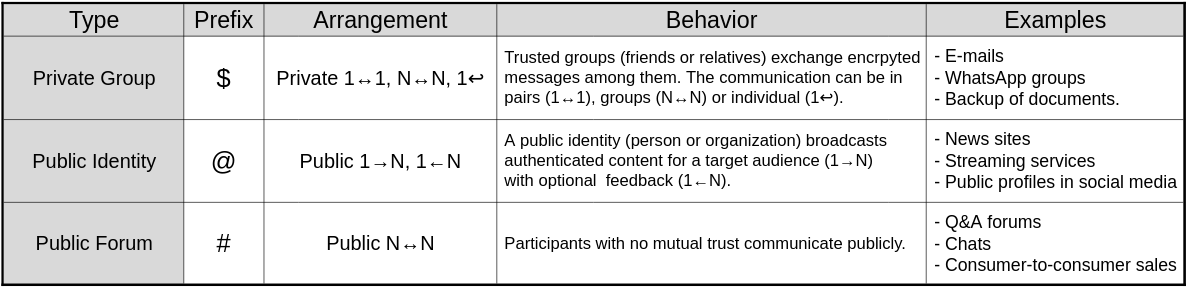
\includegraphics[width=\textwidth]{arrangements.png}
\caption{The three types of chains and arrangements in \FC.}
\label{fig.table}
\end{figure*}

In Section~\ref{sec.freechains}, we introduce the basic functionalities of \FC
to create and disseminate posts.
In Section~\ref{sec.consensus}, we describe the consensus algorithm with its
goals, incentives, and possible attacks and mitigations.
In Section~\ref{sec.related}, xxx.
In Section~\ref{sec.conclusion}, yyy.

\section{Freechains}
\label{sec.freechains}

\FC is an unstructured peer-to-peer topic-based publish-subscribe system.
Each topic, or \emph{chain}, is organized as a \emph{Merkle DAG}, i.e., a
directed acyclic graph immune to modifications.
The chain DAG is disseminated peer by peer in the network with gossiping.
This way, as an author posts to a chain, other users subscribed to the same
chain eventually receive the message.
\FC supports multiple types of chains with different arrangements of public and
private communication, which are detailed in Figure~\ref{fig.table}.
In this section, we operate a private group to describe the basic behavior of
chains.
At the end of the section, we also exemplify a public identity chain.
In Section~\ref{sec.consensus}, we detail the behavior of public forums, which
involve untrusted communication between users and require the proposed
reputation and consensus mechanisms.

All \FC operations go through a \emph{daemon} (analogous to Bitcoin full nodes)
which validates posts, links them in the Merkle DAGs, persists the chains in
the disk, and communicates with other peers in the network to disseminate the
graphs.
The command that follows starts a daemon to serve further operations:

{\footnotesize
\begin{verbatim}
 > freechains-daemon start "/var/freechains/"
\end{verbatim}
}

The actual chain operations use a separate client to communicate with the
daemon.
The next sequence of commands (i) creates a shared key, (ii) joins a private
group chain (prefix $\$$), and (iii) posts a message in the chain:

{\footnotesize
\begin{verbatim}
 > freechains crypto shared "strong-password" # (i)
 A6135D..
 > freechains "$family" join "A6135D.."       # (ii)
 42209B..
 > freechains "$family" post "Good morning!"  # (iii)
 1_EF5DE3..
\end{verbatim}
}

\begin{figure}[t]
\centering
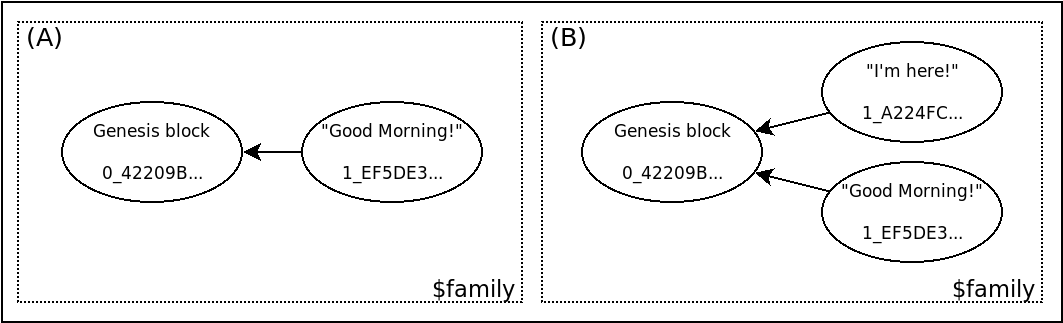
\includegraphics[width=0.5\textwidth]{family.png}
\caption{Two DAG configurations. (A) has a single head pointing to the
genesis block. (B) has a fork with two heads pointing to the genesis block.}
\label{fig.family}
\end{figure}

A private chain requires that all participants use the same shared key when
joining the group.
A \emph{join} only initializes the DAG locally in the file system, and a
\emph{post} also only modifies the local structure.
No communication occurs at this point.
Figure~\ref{fig.family}.A depicts the state of the chain after the first post.
The genesis block with height $0$ and hash \texttt{42209B..}
depends only on the arguments given to \emph{join}.
The next block with height $1$ contains the posted message, and its hash
\texttt{EF5DE3..} depends on its payload and hash of previous block, complying
with the Merkle~DAG.

\FC adheres to the \emph{local-first} software principle~\cite{p2p.local},
allowing networked applications build on top of it to host their own data and
work locally while offline.
Except for synchronization, all other operations in the system only affect the
local replica.
In particular, joining a chain with the same arguments in another peer results
in the same genesis state, even if the peers have never met before.
Hence, before synchronizing, others peers have to initialize the chain with the
same steps:

{\footnotesize
\begin{verbatim}
 > freechains-daemon start "/var/freechains/"
 > freechains crypto shared "strong-password"
 A6135D..
 > freechains "$family" join "A6135D.."
 42209B..
\end{verbatim}
}

Synchronization is explicit, in pairs, and unidirectional.
The next command asks daemon in \emph{localhost} to connect to daemon in
\emph{remote-ip} and receive all missing blocks from there:

{\footnotesize
\begin{verbatim}
 > freechains "$family" recv "<remote-ip>"
 1/1 # one block received from <remote-ip>
\end{verbatim}
}

The complementary command \emph{send} synchronizes the DAGs in the other
direction.
Note that \FC does not construct a network topology or synchronize peers
automatically.
There are no preconfigured peers, no \emph{root servers}, no peer discovery.
All connections happen through the \emph{send} and \emph{recv} commands which
have to specify the peers explicitly.
In this sense, the protocol only gives basic support for communication in pairs
of peers and any further automation requires external tools.

The next sequence of commands checks the hash(es) of the block(s) at the head
of the DAG (the latest blocks), and then reads the payload of the single head
found:

{\footnotesize
\begin{verbatim}
 > freechains "$family" heads
 1_EF5DE3..
 > freechains "$family" payload "1_EF5DE3.."
 Good morning!
\end{verbatim}
}

Now the new peer is in the same state as the original peer in
Figure~\ref{fig.family}.A.
However, since the network is inherently concurrent and users are encouraged to
work locally, typical graphs are not lists, but DAGs with multiple heads.
As an example, suppose the new peer posts a new message "I'm here!" before the
\emph{recv} above, when the local DAG is still in its genesis state.
In this case, as illustrated in Figure~\ref{fig.family}.B, the resulting graph
after the synchronization now would contain two blocks with height $1$.
%
Forks create ambiguity when trying to order messages in a conversation.
Private chains can apply simple methods to reach consensus, such as relying on
the blocks timestamps.
However, in public forums, malicious users could modify their local time to
affect new block timestamps and manipulate the order of messages.

To conclude the basic chain operations, users can rate posts with \emph{likes}
and \emph{dislikes}, which can be consulted later:

{\footnotesize
\begin{verbatim}
 > freechains "$family" like "1_EF5DE3.."
 2_BF3319..
 > freechains "$family" reps "1_EF5DE3.."
 1  # post received 1 like
\end{verbatim}
}

In private groups, likes are unlimited and behave much like in centralized
systems.
In public forums, however, likes are restricted, have to be signed by users,
and are at the core of the consensus algorithm.

For the sake of completeness, \FC also supports public identity chains (prefix
$@$), which relies on public-key cryptography to attach an identity to a chain
and to verify the authenticity of posts:

{\footnotesize
\begin{verbatim}
 > freechains crypto pubpvt "other-password"
 EB172E.. 96700A..
 > freechains "@EB172E.." join
 F4EE21..
 > freechains "@EB172E.." post "This is Pele" \
    --sign=96700A..
 1_547A2D..
\end{verbatim}
}

In the example, a public figure creates a pair of public/private keys and joins
an identity chain attached to his public key.
Every post in this chain needs to be signed with the associated private key to
be accepted in the network.

\section{The Consensus Algorithm}
\label{sec.consensus}

In the absence of moderation, peer-to-peer public forums are impractical.
At the root of the problem lies Sybil attacks, which use large numbers of fake
identities to abuse the system.
In permissionless peer-to-peer systems, creating an identity is as simple as
generating a pair of public/private keys, taking a few seconds to generate
hundreds of identities to post thousands of SPAM messages in the system.
Hence, without moderation, there are no limits on the number and size of posts
and no reasonable policy to distinguish quality.

\subsection{Overall Design}

We propose a reputation system that works together with a consensus algorithm
to make peer-to-peer public forums practical.
%
The reputation system uses tokens named \reps to rate content:
a \emph{like} operation is a positive feedback that helps subscribers find good
content amid excess;
a \emph{dislike} operation is a negative feedback that revokes content when
crossing a threshold.
%
Without restrictions, like operations alone are not satisfactory, specially
with considering hypothetical Sybils abusing the system.
Therefore, \reps must be subject to some sort of scarcity that demands
non-trivial work immune to automation.
Bitcoin employs CPU proof-of-work as a solution for Sybils, but in our context,
content authoring is already an intrinsic human work that we can take
advantage.
In our system, content authoring is the only operation that can generate \reps,
%but limited by periods of time to prevent excess (e.g., once in a day per user).
%Additionally,
while likes and dislikes only transfer \reps between users, preserving
scarcity.
%
However, like operations and scarcity are still not enough as they call for
consensus in the network: now we need to track the reputation of users to check
if they are allowed to post new messages or spend likes.
Since posts and like operations are concurrent in the network, we need to
figure out how to order them consistently across all peers so that they
converge to the same state.

\begin{figure}[t]
\centering
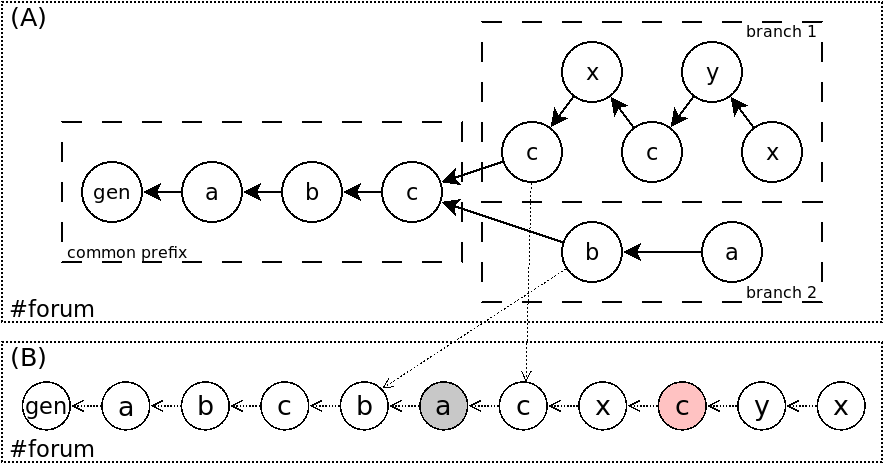
\includegraphics[width=0.49\textwidth]{reps2.png}
\caption{
    (A) A public forum DAG with a common prefix and two branches.
    (B) Hypothetical corresponding total order between blocks.
}
\label{fig.reps}
\end{figure}

\begin{figure*}[ht]
\centering
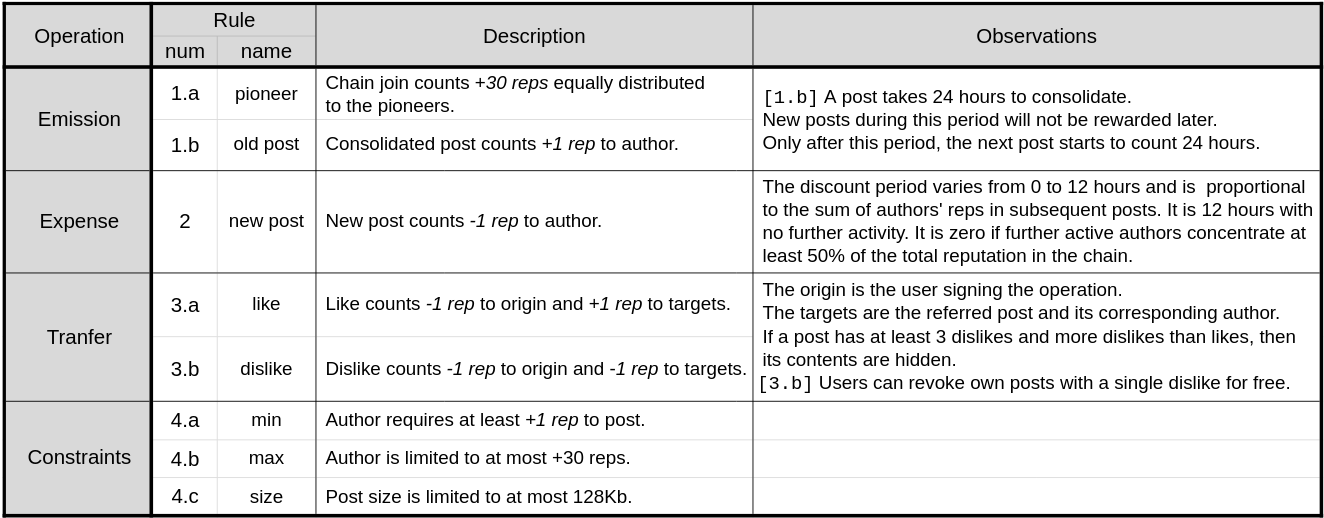
\includegraphics[width=\textwidth]{rules.png}
\caption{Reputation rules for public forum chains.}
\label{fig.rules}
\end{figure*}

Our solution is to preserve the order seen by the users constituting the
majority of reputation, which are more likely to be non malicious.
%
Figure~\ref{fig.reps}.A illustrates the reputation criterion.
%, still abstractly, since we did not discuss the actual rules for content creation and rating.
A public chain DAG has a common prefix with signed posts from users $a$, $b$,
and $c$.
Let's assume that within the prefix, users $a$ and $b$ have contributed with
more content and have more reputation combined than $c$ has alone.
%
After the prefix, the chain forks in two branches:
in \emph{branch 1}, only user $c$ remains active and we see that new users $x$
and $y$, with no previous reputation, generate a lot of new content;
in \emph{branch 2}, only users $a$ and $b$ exist but with less activity.
Nonetheless, \emph{branch 2} takes priority because, at the forking point, $a$
and $b$ have more reputation than $c$, $x$, and $y$ combined.

\begin{comment}
Our sequencing proposal is straightforward and compares the sum of \reps
accumulated in the past by the authors in pairs of concurrent branches.
Consensus is still required because like operations spend \reps that need
to be verified consistently by all peers in the network.
To verify operations in concurrent branches, the graph must be sequenced to
generate a total order between blocks.
The branch with more reputation---the one with more work---prefixes the
sequence as a whole.
If the suffixed branch has a conflicting operation (e.g., a like from a user
without reputation), then this operation and all remaining blocks are removed
from the DAG.
\end{comment}

Figure~\ref{fig.reps}.B indicates the consensus order between blocks in the
chain.
All operations in \emph{branch 2} are accounted before any operation in
\emph{branch 1}.
Note that the common prefix also had a fork that favored $a$.
%
At any point in the consensus timeline, if an operation fails, all remaining
blocks are removed from the chain DAG.
As an example, suppose the last post by $a$ (in gray) dislikes user $c$,
decreasing its reputation.
Then, it's possible that the last post by $c$ (in red) is rejected together
with all posts by $y$ and $x$ in sequence.
%
Unlike Bitcoin, forks are not only allowed but encourage by the local-first
principle.
The resulting linked list is only a view of the primary DAG structure.
However, the longer a peer remains disconnected, the more conflicting
operations it performs, the higher is the probability of rejection when
rejoining.

Some other considerations about merging forks:
Peers that saw branches with less reputation first (\emph{branch 1}) need to
recompute everything starting at the forking block.
This might involve reorganizing or even removing content in the end user
software.
This behavior is similar to chain reorganization in Bitcoin when a peer detects
a new longest chain and disconsiders old blocks.
%
Likewise, peers that saw branches with more reputation first (\emph{branch 2})
just need to sequence the other branch and do not need to recompute anything.
This behavior is reasonable and expected to happen in all peers connected with
the majority of the network.

\begin{comment}
As a last remark, let's assume that user $c$ is malicious and is trying to use
Sybils $x$ and $y$ to multiply content generation during a certain period and
collect enough \reps in separate of the network to perform an attack later.
Even though the blocks of \emph{branch 1} would appear after \emph{branch 2},
they could still be successful to collect the intended \reps.
However, if the majority of the network in \emph{branch 2} notices that the
messages in \emph{branch 1} are malicious, they can still defend themselves:
Since they have more reputation Users $a$ and $b$ can pretend that they did not see \emph{branch 1} and post
dislikes to $c$ at the end of \emph{branch 2} which .
\end{comment}

\subsection{Public Forum Chains}

In \FC, public forums follow strict rules that track the reputation of users in
order to enforce consensus and content moderation.
Users in public forums need to sign their posts in order to be accounted by the
reputation system and operate in the chains.
The rules are specified in Figure~\ref{fig.rules} and are explained as follows.

Rule~\texttt{1.a} bootstraps a chain assigning \nreps{30} to the pioneer
referred in the \emph{join} command.
The commands that follow create an identity whose public key is assigned as the
pioneer in the public chain.
The first post is signed by the pioneer and indicates the purpose of the chain:

{\footnotesize
\begin{verbatim}
 > freechains crypto pubpvt "pioneer-password"
 4B56AD.. DA3B5F..
 > freechains "#forum" join "4B56AD.."
 10AE3E..
 > freechains "#forum" post --sign=DA3B5F.. \
    "The purpose of this chain is..."
 1_CC2184..
\end{verbatim}
}

The pioneer shapes the initial culture of the chain with its first posts, while
he gradually transfers \reps to other authors, which transfer to other authors,
expanding the community.
%
Note that chains with the same name but different pioneers are incompatible
because the hash of genesis blocks also depend on the pioneers' public key.

Our most basic concern in public forums is to resist Sybils spamming the chains
with new posts.
Fully peer-to-peer systems cannot rely on identity validations or CAPTCHAs due
to the lack of a central authority.
Other alternatives include relying on social trust graphs, in which users
already in the community vouch for new users, or imposing economic costs to new
posts, such as solving a proof-of-work puzzle.

We propose a mix between the last two approaches with the basic premise that
users with no previous reputation are not allowed to post.
Rule~\texttt{4.a} states that authors require at least \onerep to post, while
rule~\texttt{2} states that new posts cost \onerep, even from existing users.
These rules combined prevents Sybils to abuse the system.
Rule~\texttt{3.a} allows an existing user to like a new user's post, which
unblocks the post and vouches for the new user, but also at the cost of
\onerep.
These rules impose costs not only for welcoming new users, but also for posting
new messages, which also prevents abuse from malicious users already in the
chain.
%
Note that the pioneer rule~\texttt{1.a} solves a chicken-and-egg problem in
which the first new author would require \reps from non-existing previous
authors.
%
In the commands that follow, a new user joins the same public chain and posts a
new message, which is welcomed with a like signed by the pioneer:

{\footnotesize
\begin{verbatim}
 > freechains crypto pubpvt "new-author-password"
 503AB5.. 41DDF1..
 > freechains "#forum" join "4B56AD.."
 10AE3E..
 > freechains "#forum" post --sign=41DDF1.. \
    "I'm a newbie..."
 2_C3A40F..
 > freechains "#forum" like "2_C3A40F.." \
    --sign=DA3B5F..
 3_59F3E1..
\end{verbatim}
}

\begin{figure}[ht]
\centering
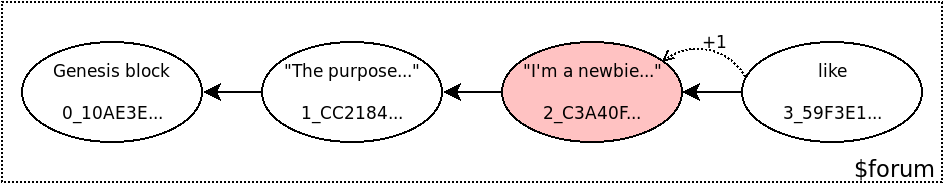
\includegraphics[width=0.49\textwidth]{forum.png}
\caption{
    The \texttt{like} approved the newbie message into the \texttt{\#forum} DAG.
}
\label{fig.forum}
\end{figure}

Figure~\ref{fig.forum} illustrates the chain DAG up to the like operation.
The pioneer started with \nreps{30} (rule~\texttt{1.a}) and posted an
initial message, reducing his balance to \nreps{29} (rule~\texttt{2}).
Then, a new user with \nreps{0} tried to post a message
(hash~\texttt{C3A40F..}), which was initially blocked (rule~\texttt{4.a}), as
the red background suggests.
Then, the pioneer likes the \emph{newbie} message, which reduces his balance to
\nreps{28} and increments new user's to \onerep (rule~\texttt{3.a}, which is
immediately consumed by the blocked post.
At the end, the pioneer has \nreps{28} and the new user remains with \nreps{0}
but with his post accepted.
Note that the overall balance is -\nreps{2} from the penalties in the two post
operations (rule~\texttt{2}).
After at most 12 hours, these penalties are dismissed and the \nreps{2} are
recovered (rule~\texttt{2}):
    the pioneer goes to \nreps{29} and the new user to \onerep, which sum up to
    the pioneer's original \nreps{30}.

With no additional rules to generate \reps, the initial \nreps{30} would
constitute the whole ``chain economy'' forever.
In order to stimulate content creation and grow the economy of chains,
rule~\texttt{1.b} awards authors with \onerep 24 hours after each post.
This period allows other users to judge the post before awarding the author,
and also regulates the growth speed of the chain.
Hence, 24 hours after the commands above, the pioneer would accumulate
\nreps{30} and the new user \nreps{2}, growing the total chain amount in
\nreps{2} as result of the two consolidated posts.
Rule~\texttt{1.b} awards at most one post per day per author, i.e., with 10
posts in 7 days an author would collect \nreps{7}.
Note that rule~\texttt{4.b} limits authors to at most \nreps{30}, which
incentivizes them to spend likes and promotes decentralization in the network.

Likes and dislikes (rules \texttt{3.a} and \texttt{3.b}) serve three purposes:
    (a) welcoming new users, (b) measuring the quality of posts, and
    (c) censoring abuse (SPAM, fake news, illegal content).
%
The reputation of a given post is the difference between its likes and
dislikes, which can be used for end-user software for filtering and
highlighting purposes.
%
The quality of posts is subjective and is up to users to judge with likes,
dislikes, or simply abstaining.
On the one hand, since \reps are finite, users need to ponder and avoid
indiscriminate expenditure.
On the other hand, \reps limited to at most \nreps{30} per author and expire
after 90 days (rules~\texttt{4.b} and~\texttt{4.c}).
The scarcity and limits work together towards the chain quality.
%
Note that a dislike shrinks the chain economy since it removes \reps from both
the origin and target.
The contents of a post may be hidden by the network, as detailed next, if it
has at least 3 dislikes and the number of dislikes is higher than the number of
likes.
Considering that \reps are scarce, dislikes are more directed to combat abuse,
but not to eliminate divergence of opinion.

\begin{figure}[ht]
\centering
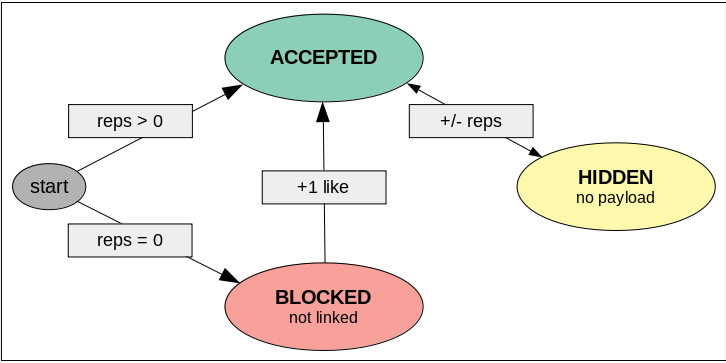
\includegraphics[width=0.49\textwidth]{state.png}
\caption{
    State machine of posts:
    \emph{BLOCKED} posts are not linked in the DAG.
    The payload of \emph{HIDDEN} posts are not retransmitted.
    \emph{ACCEPTED} posts are linked and retransmitted.
}
\label{fig.state}
\end{figure}

A post has three possible states: \emph{BLOCKED}, \emph{ACCEPTED}, or
\emph{HIDDEN}.
Figure~\ref{fig.state} specifies the transitions between the states.
%
If the author has reputation, the post is immediately accepted.
Otherwise, it is blocked and requires a like from another user.
Blocked posts are not considered part of the chain DAG in the sense that new
posts do not link back to it.
%
Peers are not required to hold blocked posts and neither retransmit them to
other peers.
However, if they do not reach other users, they will never have the chance to
be welcomed with a like.
A reasonable policy for blocked posts is to hold them in a temporary queue and
retransmit them to a small extent for some visibility.
%
Once accepted, the post becomes part of the chain and can never be removed
again since Merkle DAGs are immutable by design.
Note that blocked posts that become accepted must always be succeeded by a
\emph{like} (Figure~\ref{fig.forum}).
%
If the number of dislikes exceed the threshold, the post payload becomes
hidden, i.e., it is not retransmitted to other peers and should be removed from
local storage.
The Merkle DAG depends only on the hash of the payload, so it is not a problem
to hide it since the DAG itself contains the dislikes that prove the state of
the post.
Also, if the post receives new likes and changes its state, it means that the
payload is still known somewhere and peers can request it when synchronizing
again.

\subsection{TODO}

- users that work twice, bots

Terminar com "@!xxx" dizendo que vale reps mas que owner pode "intervene"

- summary
    - parallel w/ bitcoin
        - ponte entre reputacao -> sybil -> consenso
    - no problem w/ forks

We reach a similar solution to Bitcoin but adapted to our domain
- we need consensus to make the reputation system work
- we need reputation system to reach consensus
- same virutous cycle as bitcoin

The more CPU work is done, the stronger becomes the proposal, the more peers
follow it, the more tokens are mined.
There is a strong association between work, profit and consensus that enables
Bitcoin as a peer-to-peer cash system.

- reputation system to rate messages
    - positively (to distinguish from excess), or
    - negatively (to block SPAM, fake news, illegal content)
- some sort of scarcity (work)
    - you like you loose
    - you work you get
    - otherwise sybil, "likes" abuse
    - incentives for continuous, good quality posts
- consensus to ???

\section{Related Work}
\label{sec.related}

Bitcoin employs CPU proof-of-work as a solution, but did not solve the
centralization issue completely because the cost to perform work is not
equally distributed
(depends on costs of equipment and energy)
    - bitcoin demands connectivity to avoid forks
    - forks ok in freechains since operations are not critical and can be reverted
    - 50+1 attack easy in first nodes if not all nodes keep participating
        - freechains requires checkpoints

- related work public forums in scuttlebutt are permissioned (you decide who
  participates). each user has a completely different view of \#chat. not really
  public although some intersections
    - you can see an answer but not a question, or a question w/ no answers
      even if the best answer exists. no content discovery



\section{Conclusion}
\label{sec.conclusion}


Like \emph{bitcoins}, \reps are scarce, hard to generate, and easy to verify.
Unlike \emph{bitcoins}, \reps .


With this design, we retarget  , the balance between work, profit and consensus also applies 

attack 50+1 but not as
cite local-first software

 (crypto proof \& authoring),
while verification is cheap


requires work but evaluation


, but
are evaluated by other user
The system also imposes incentives to rate posts and 

Unlike bitcoin

Since likes and dislikes spend reputation, \emph{creps} are scarce resources
Incentives to post and rate content.

There is a strong association between work, profit and consensus that enables
Bitcoin as a peer-to-peer cash system.

distinguish SPAM from legitimate
Another problem CPU



content.



 (e.g., posts on social media, public conversations
based on the reputation of users
in the network.


biggest difference:
work is subjective as is the evaluation by other users


 with consensus since
whoever proposes the ordering will choose one of the operations arbitrarily


 which is similar to the
example above (\emph{buy X} vs \emph{buy Y})

spent

with work



this gives consensus with total order, solves double spend, which is equivalent
to solving X/Y is decided above

we borrow token, scarcity


 that requires work to 
Only one purpose


- incentive
- security

- Last-Write-Wins

- just all tokens are the same, no subjective judgment, for example on why token is being transferred


 and xx timestamps.


 of the service and , and trust from users to deal

In a decentralized setting, 
    - spam
    - abuse
    - on topic
    - disconnections
    - order

Bitcoin

responses would




n user posts 

- discovery
- also consensus, ensure that participants receive all data in a consistent order
- bitcoin, discovery even disconnected, consensus, but not quality


Regardless of the Internet growth over the years,

\subsection{Subsection Heading Here}
Subsection text here.

\subsubsection{Subsubsection Heading Here}
Subsubsection text here.

\section{Conclusion}
The conclusion goes here.

\bibliographystyle{IEEEtran}
\bibliography{tpd-21}

\begin{IEEEbiography}{Michael Shell}
Biography text here.
\end{IEEEbiography}

\begin{IEEEbiographynophoto}{John Doe}
Biography text here.
\end{IEEEbiographynophoto}

\begin{IEEEbiographynophoto}{Jane Doe}
Biography text here.
\end{IEEEbiographynophoto}

\end{document}
